A fines de abril de 2014, Nvidia envió la placa de desarrollo Nvidia Jetson TK1 que contenía un SoC Tegra K1 en la variante T124.

\begin{figure}[H]
  \centering
  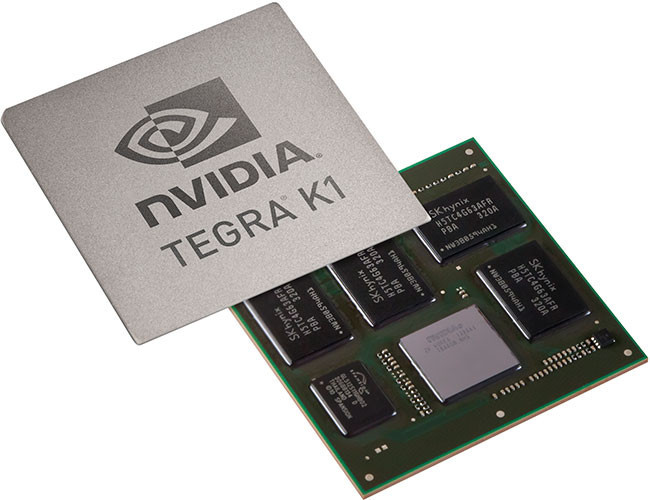
\includegraphics[scale = 0.3]{Imagenes/tegra_k1.jpg}
  \caption{Placa NVIDIA TEGRA K1}{Fuente: Internet}
\end{figure}

La placa de desarrollo Nvidia Jetson TX1 incorpora un Tegra X1 del modelo T210.

La placa Nvidia Jetson TX2 incorpora un Tegra X2 de microarquitectura GP10B. Esta placa y la plataforma de desarrollo asociada se anunciaron en marzo de 2017 como un diseño de tarjeta compacto para escenarios de bajo consumo, por ejemplo, para su uso en drones con cámara más pequeños.

El Nvidia Jetson Xavier se anunció como un kit de desarrollo a fines de agosto de 2018. Se dieron indicios de que se debería esperar una aceleración de 20 veces para ciertos casos de aplicación en comparación con los dispositivos predecesores, y que la eficiencia energética de la aplicación se mejora 10 veces.

\begin{figure}[H]
  \centering
  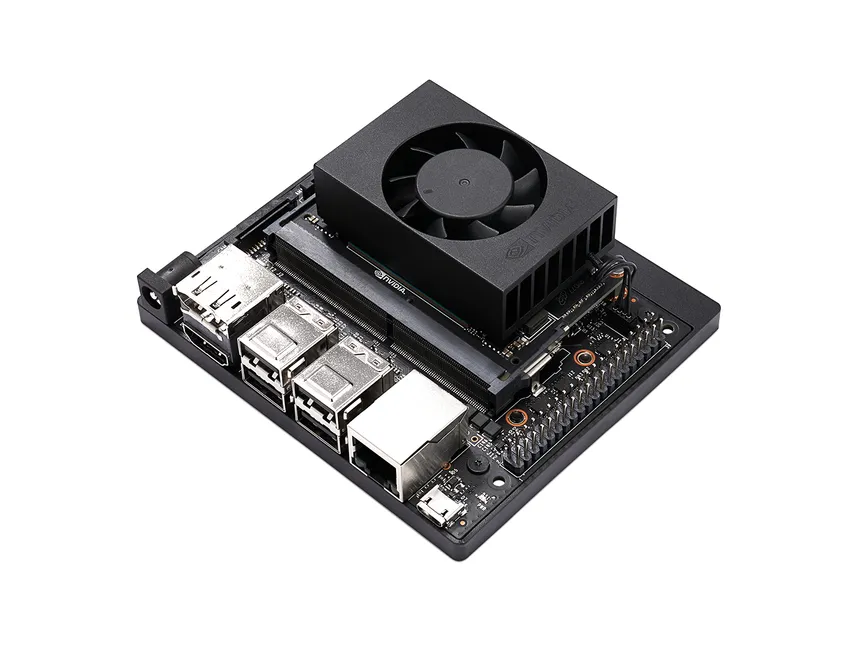
\includegraphics[scale = 0.3]{Imagenes/jetson_xavier.png}
  \caption{Placa NVIDIA Jetson Xavier}{Fuente: Internet}
\end{figure}

El Nvidia Jetson Nano se anunció como un sistema de desarrollo a mediados de marzo de 2019. El mercado previsto es la robótica para aficionados debido a su bajo precio.

\begin{figure}[H]
  \centering
  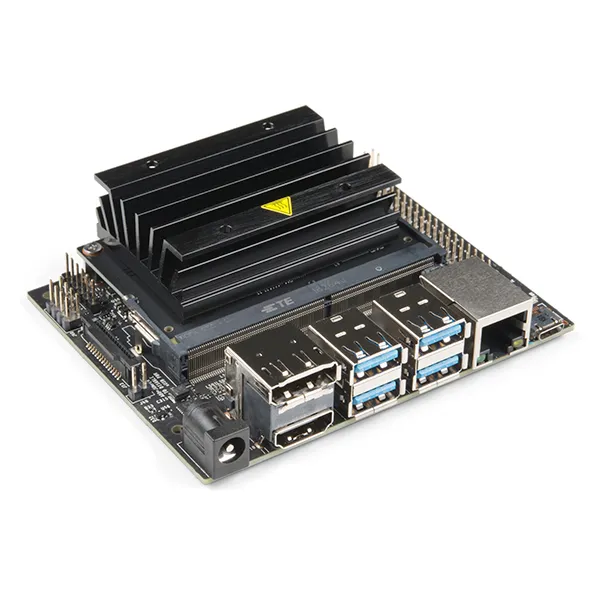
\includegraphics[scale = 0.3]{Imagenes/jetson_nano.png}
  \caption{Placa NVIDIA Jetson Nano}{Fuente: Internet}
\end{figure}

En septiembre de 2022, Nvidia anunció el Jetson Orin Nano.